\subsection{Density Profiles}

Density histograms of simulated interfaces have been used in previous publications to show ionic and molecular distribution behavior in various systems.\cite{Chang1995,Eggimann2008,Du2008,Wick2006c,Petersen2005a,Hore2008,Walker2006b,Walker2007b} In this work the density profile of water throughout the interface is fit to a hyperbolic tangent function\cite{Wick2006c,MATSUMOTO1988} as shown here:

\begin{equation}\label{tanh_fit}
	\rho(z) = \frac12(\rho_1+\rho_2) - \frac12\left(\rho_1-\rho_2\right)\tanh\left(\frac{z-z_0}{d}\right)
\end{equation}

Equation (\ref{tanh_fit}) relates the interfacial density, $\rho$, as a function of position, $z$, along a given system reference axis, to the densities of the phases, $\rho_1$ and $\rho_2$, on either side of the Gibb's dividing surface (GDS), $z_0$. The interfacial width, $d$, is related to the ``90-10'' thickness that is often reported by $t_{90-10} = 2.197d$.

These measures of interfacial thickness provide a means of comparing the depths to which the water phase is affected by ions located at the interface. The density distributions of the salts depict concentration and depletion phenomena throughout the interfacial region, and also serve to illustrate ionic surface affinity within this region. Previous work has been performed on the \airwat~interface with ions of different levels of interfacial affinity, with the more polar ions being the most interfacially active.\cite{Luo2006,Petersen2006,Petersen2005a,Allen2009,Hofft2006,Beattie2005,Bian2009,Dang2004b} We present the density distribution results for the neat \ctcwat~and salt solutions adjacent to an organic \ctc~phase. 

\subsection{Molecular Orientation}

Several methods have been used previously to show molecular orientation profiles of water molecules throughout simulated interfacial regions.\cite{Wick2006c,Thomas2007,Wick2008a,Wick2007,Fan2009,Galamba2008,Ishiyama2007,Hore2007,Hore2008} Studies have utilized various internal coordinate definitions and a number of angle definitions, orientational order parameters, and probability distributions to relate molecular, or averaged, orientations. In this work we have chosen to compute the orientation of water using two vectors that intuitively describe the orientation in space, given the locations of the three atoms comprising the molecule. The molecular bisector, a vector that points along the axis of symmetry of the water molecule from the hydrogen-end to the oxygen, provides directional orientation similar to the water molecule's dipole. A second vector, that is referred to here as the molecular normal vector, is established as the vector pointing normal to the plane formed by the three atoms of the water molecule and establishes its planar ``tilt''. Analyzing the angle made between these two vectors and a given space-fixed reference axis (herein defined as the long-axis of the simulation cells, oriented perpendicular to the interfacial plane and pointing out of the aqueous phase) is a means of finding the orientation of waters within these simulated systems as illustrated in Figure \ref{fig:water-angles}. The angle formed between the molecular bisector and the reference axis will hereafter be referred to as $\theta$, and the angle between the reference axis and the molecular normal vector as $\phi$. The analysis in this work reports the cosines of these two angles, and because of the symmetry of the water molecule where the hydrogens are not uniquely identified, the cosines of the two angles are limited as follows: $-1\le\cos\theta\le1$ and $0\le\cos\phi\le1$. We report the orientation profiles of $\theta$ and $\phi$ as functions of the distance from the GDS of the interface, as found from the fitting in our density profile analyses.

\begin{figure}[h!]
\begin{center}
	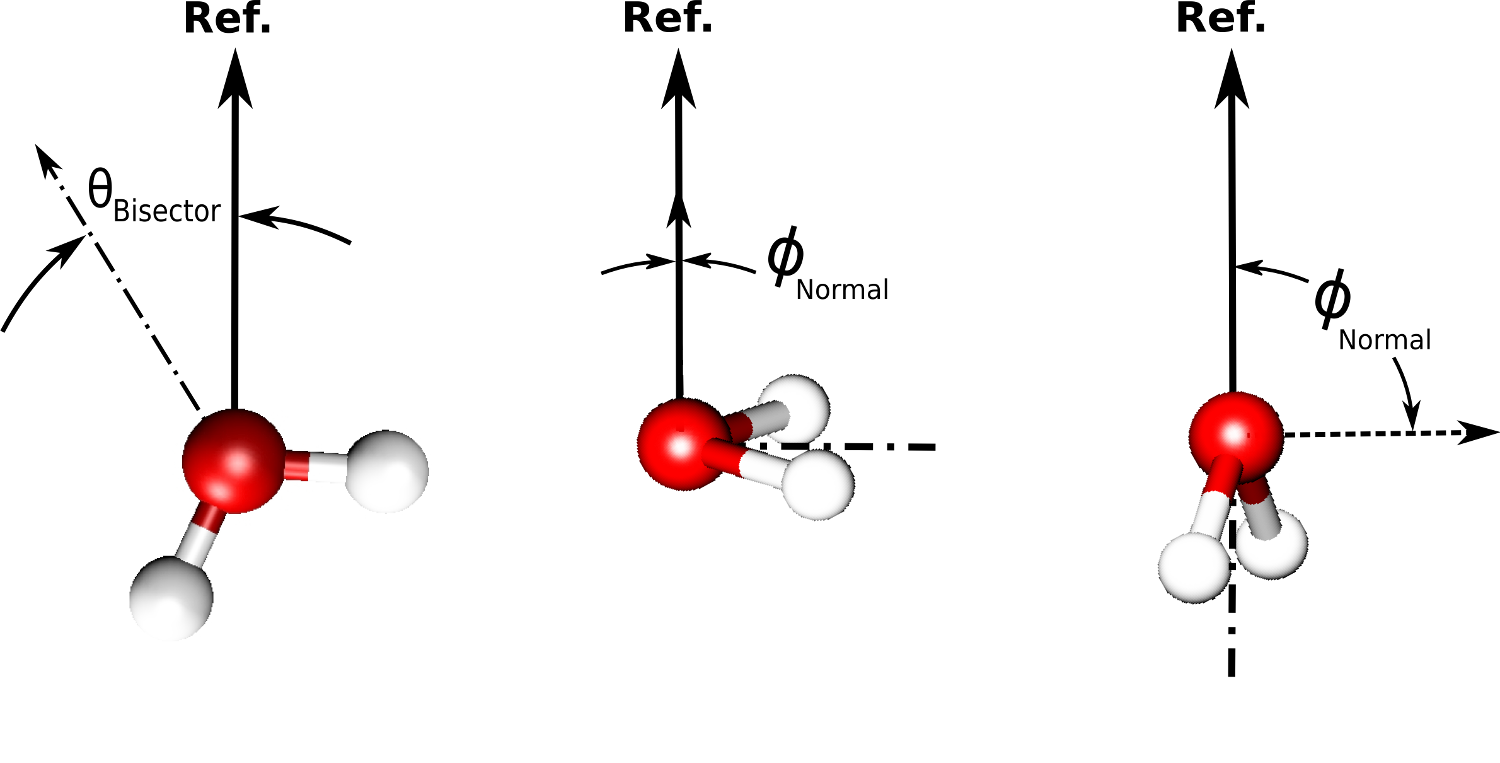
\includegraphics[scale=1.0]{images/water-angles.png}
	\caption{Angles used to define molecular orientation. The system reference (Ref.) axis is that which is perpendicular to the plane of the aqueous-organic interface, and points out from the aqueous phase into the organic one. The molecular bisector vector points from the hydrogen-end of the water to the oxygen end, and orients along the axis of symmetry. The angle it forms with the reference axis is either aligned or anti-aligned such that $-1\le \cos\theta \le 1$. The angle formed between the vector normal to the molecular plane (formed by the three water atoms) and the reference-axis orients the ``twist'' of the molecule such that $0 \le \cos\phi \le 1$, where the water molecular plane is either laying flat on the interface ($\cos\phi=1$), or the water is perpendicular to the interface ($\cos\phi=0$).}
	\label{fig:water-angles}
\end{center}
\end{figure}


\subsection{Computational SFG}

A difficult challenge for experimental surface studies is in understanding the vibrational spectroscopy of liquid water. Hydrogen bonding between water molecules causes inter- and intramolecular couplings that lead to broad spectral envelopes, each containing a distribution of water-bonded species. Simulations provide the analytical capacity to relate the broad lineshapes, and the often difficultly-assessed impact of hydrogen bonding as a function of OH vibrational frequency, to microscopic geometries, forces, and environments. In this work we compute the SFG spectra of the interface between the salt solutions and an organic phase to compare with the experimental results of similar systems.\cite{McFearin2009} 

The computational method used in this work is based on that of Morita and Hynes\cite{Morita2000} as outlined in a previous study by this group utilizing the same technique.\cite{Walker2008} The computational SFG technique has been improved in more recent studies by Morita et al,\cite{Morita2002,Ishiyama2009} and with other enhanced water models. The technique used in this work matches qualitatively the experimental spectra to a sufficient degree such that we may draw qualified conclusions about lineshape and intensity. 

